\chapter{Часть 5. Марковские цепи. Определение и построение}
\label{ch:сhap5}

Реализация:\\

\begin{figure}[ht]
    \centering
    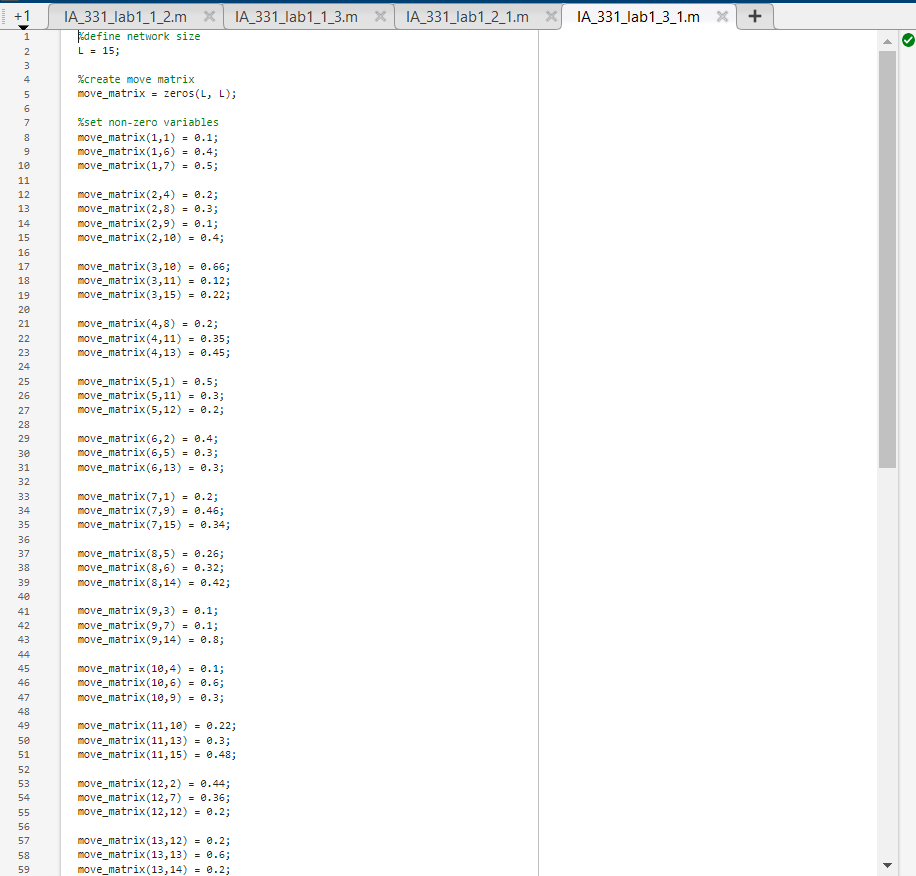
\includegraphics[width=1.0\textwidth]{IA_331_lab1_1_3p1.png}
    \caption{Реализация заданий из части 5}
    \label{fig:open_audio}
\end{figure}

\begin{figure}[ht]
    \centering
    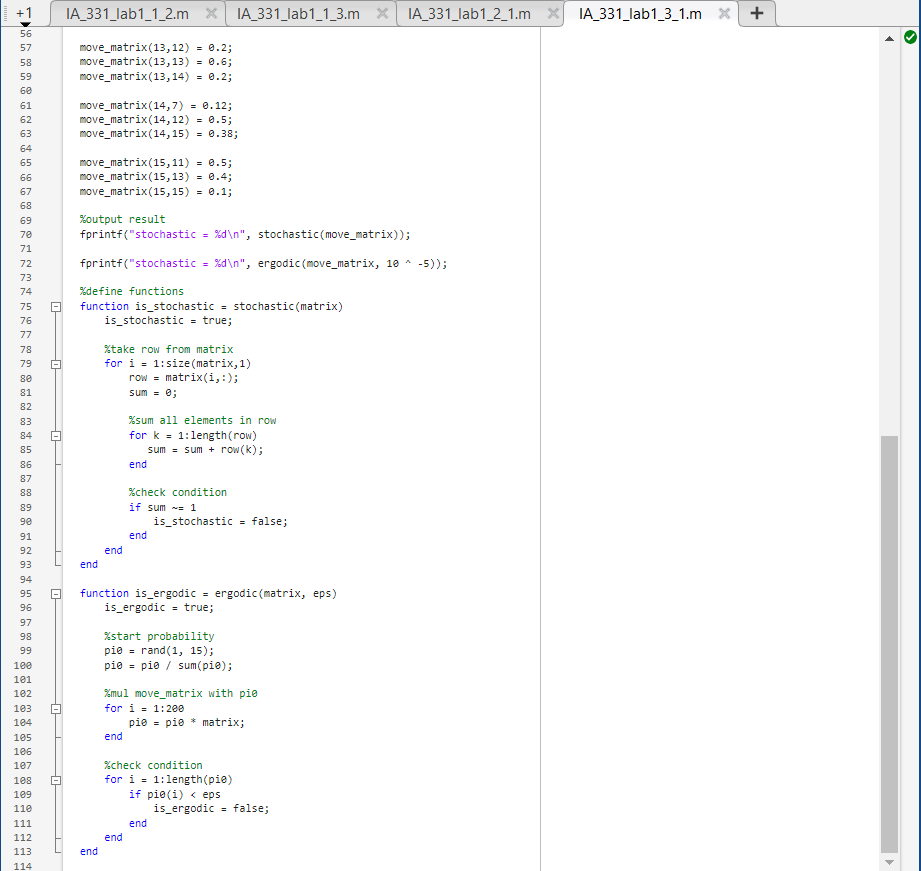
\includegraphics[width=1.0\textwidth]{IA_331_lab1_1_3p2.png}
    \caption{Реализация заданий из части 5}
    \label{fig:open_audio}
\end{figure}

Результат:

\begin{figure}[ht]
    \centering
    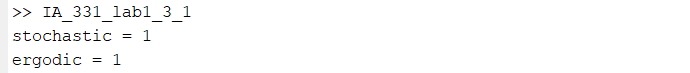
\includegraphics[width=1.0\textwidth]{IA_331_lab1_3_1_res.png}
    \caption{Результат работы программы для части 5}
    \label{fig:open_audio}
\end{figure}


\endinput